\chapter{Konzept}
\label{sec:konzept}

\section{Selektion der Disziplinen und Algorithmenen}
\label{sec:konzept:disziplin-und-algorithmen}
Im \cref{sec:recherche} wurden Disziplinen und Algorithmen erläutert. In diesem Abschnitt wird erläutert wie diese Auswahl getroffen wurde auf Basis der Anforderungen aus \cref{sec:anforderungsanalyse}.

\subsection{Einschränkung der Data Mining Disziplinen}
\label{sec:konzept:disziplinauswahl}
Ziel dieser Arbeit ist es, Attribute von Objekten zu eruieren, welche in einer Gruppe von Buchungen oft vorkommen\todo{cref zu Kapitel 1}. Nachfolgend wird anhand dieser Aufgabenstellungen entschieden, welche Disziplinen im Data Mining (siehe \cref{sec:recherche:dataminingtechniken:disziplinen} \nameref{sec:recherche:dataminingtechniken:disziplinen}) sich dazu eignen. Als Grundlage der Entscheidung gelten die Anforderungen welche an die Algorithmen gestellt wurden (siehe \cref{sec:anforderungsanalyse:algorithmen} \nameref{sec:anforderungsanalyse:algorithmen}).

\subsubsection{Association rule learning}
\label{sec:konzept:disziplinauswahl:association}
Mittels Association rule learning (siehe \cref{sec:recherche:dataminingtechniken:disziplinen:association} \nameref{sec:recherche:dataminingtechniken:disziplinen:association}) lassen sich aus allen selektierten Buchungen die Häufigkeiten von Attributkombinationen herausfinden. Dadurch kann die Fragestellung beantwortet werden (siehe \cref{sec:einletung:ziel} \nameref{sec:einletung:ziel}).


\subsubsection{Classification}
\label{sec:konzept:disziplinauswahl:classification}
Bei der Classification handelt es sich um ein \gls{supervisedlearning} (siehe \cref{sec:recherche:dataminingtechniken:disziplinen:classification} \nameref{sec:recherche:dataminingtechniken:disziplinen:classification}). Deshalb sind vorab Klassen zu definieren welche den Objekten zugewiesen werden. Diese Informationen sind jedoch noch nicht vorhanden, weshalb in den Anforderungen (siehe \cref{sec:anforderungsanalyse:algorithmen:resultat} \nameref{sec:anforderungsanalyse:algorithmen:resultat}) ein \gls{unsupervisedlearning} Algorithmus vorausgesetzt wurde. Deshalb eignet sich die Classification für diese Aufgabenstellung nicht.

\subsubsection{Lineare Regression}
\label{sec:konzept:disziplinauswahl:regression}
Linere Regression Algorithmen suchen eine Formel, damit man von einer abhängiger Variable auf unabhängige Grössen schliessen kann (siehe \cref{sec:recherche:dataminingtechniken:disziplinen:regression} \nameref{sec:recherche:dataminingtechniken:disziplinen:regression}). Damit kann man bei den Interhome Daten für neue Buchungen Attribute voraussagen. zum Beispiel wenn man die Kreditwürdigkeit von Kunden überprüfen möchte auf Basis von alten Buchungen.

Diese Algorithmen eignen sich jedoch nicht für diese Arbeit, da weder Attribute noch Gruppen von Buchungen zurückgeliefert werden (siehe \cref{sec:anforderungsanalyse:algorithmen:resultat} \nameref{sec:anforderungsanalyse:algorithmen:resultat}).

\subsubsection{Cluster analysis}
\label{sec:konzept:disziplinauswahl:clusteranalysis}
Das Resultat einer Cluster analysis sind Gruppen (Clusters) von Buchungen, die untereinander ähnlich, und zu allen anderen Gruppen möglichst unähnlich sind (siehe \cref{sec:recherche:dataminingtechniken:disziplinen:clusteranalysis} \nameref{sec:recherche:dataminingtechniken:disziplinen:clusteranalysis}). Da die Instanzen innerhalb des Clusters ähnlich zueinander sind, ist zu erwarten dass eine Häufigkeitszählung der Attribute innerhalb der Clusters aufzeigt, welche Eigenschaften besonders oft miteinander gebucht werden. Deshalb wird zuerst ein Clustering durchgeführt und anschliessend der Apriori Algorithmus auf jedem Cluster ausgeführt. 

Dies erweitert die Resultate des \nameref{sec:konzept:disziplinauswahl:association} (siehe \cref{sec:konzept:disziplinauswahl:association}) um die Möglichkeit, die Attributmenge in verschiedene Untergruppen aufzuteilen.

\subsubsection{Collaborative Filtering}
\label{sec:konzept:disziplinauswahl:collaborativefiltering}
Collaborative Filtering werden für recommender systems eingesetzt um dem Benutzer Instanzen vorzuschlagen die er auch mögen könnte. Grundlage für diese Entscheidungen sind seine bisherigen Interaktionen mit dem System verglichen mit denen von anderen Benutzern. Dadurch könnte bei den Interhome Daten Objekte vorgeschlagen werden die der Kunde auch mögen könnte. Es werden jedoch keine Attribute oder Instanzgruppen gebildet, womit die Anforderung \cref{sec:anforderungsanalyse:algorithmen:resultat} nicht erfüllt sind.


\subsection{Algorithmenauswahl}
\label{sec:konzept:algorithmenauswahl}
Im \cref{sec:konzept:disziplinauswahl} wurden die Disziplinen auf Association rule learning und Cluster analysis eingeschränkt und im \cref{sec:recherche:algorithmen} die einzusetzenden Algorithmen beschrieben. Nachfolgend wird beschrieben wieso jene Abläufe ausgewählt wurden.

\subsubsection{Association rule learning: Apriori}
\label{sec:konzept:algorithmenauswahl:apriori}
Das Association rule learning besteht aus zwei Schritten. Zuerst werden mittels des Apriori Algorithmus häufige Attributkombinationen gesucht und anschliessend Regeln aufgestellt um Korrelationen zwischen gemeinsam auftretenden Eigenschaften aufzuzeigen.
Der zweite Schritt wird nicht durchgeführt, da die Regeln des Association rule learning für die Aufgabenstellung dieser Arbeit nicht benötigt werden.

Es gibt Alternativen zum Apriori Algorithmus. Dies sind zum Beispiel der AprioriTid oder AprioriHybrid. Diese generieren die identischen Resultate und unterscheiden sich nur in der Laufzeit. Der AprioriTid kann zu beginn der Häufigkeitszählung bessere Leistung aufzeigen, ist jedoch langsamer gegen dessen Ende. Der AprioriHybrid verwendet zu Beginn der Apriori, und am Schluss den AprioriTid\footcite{association_rule_learning_2017-01-05}. 

Es ist noch unklar, welcher Algorithmus die besseren Laufzeiten aufweist. Zum Schluss oder nach der Arbeit kann in einer Vertiefung der AprioriTid oder der AprioriHybrid eingesetzt werden um die Leistungen der Algorithmen zu vergleichen. Im ersten Schritt wird der Apriori benutzt um zu analysieren ob die Resultate brauchbare Informationen liefern.

\subsubsection{Clustering}
\label{sec:konzept:algorithmenauswahl:clustering}
Es gibt diverse Algorithmen welche sich verschiedene Problemstellungen annehmen. Unterteilen lassen sich diese in vier Gruppen:
\begin{itemize}
	\item Partitioning
	\item Hierarchical
	\item Density-based
	\item Grid-mased
\end{itemize}
Nicht alle Algorithmen lassen sich eindeutig einer Gruppe zuweisen. Jedoch hilft diese Auflistung eine Übersicht über die Verfahren zu geben\footcite{data_mining_concepts_and_techniques}.

Für die Auswahl eines Algorithmus müssen die Charakteristiken der Daten bekannt sein, wie diese zum Beispiel verteilt (z.B. Kugel-, Kreis-, S-Förmig) oder wie viele Cluster sinnvoll sind. Diese sind bislang jedoch noch bekannt.
Partitioning- und Hierarchical-Vorgehensweisen benötigen zur Berechnung der Clustern deren Anzahl. Bei ersteren kann diese anhand der Elbow-Methode berechnet werden\footcite{elbow_method}. Bei Hierarchischen Clustern müsste man dies jedoch für jeden Ast ermittelt. Da die Laufzeit von solchen Algorithmen bereits $\mathcal{O}(k^2)$ beträgt ist diese Vorgehensweise nicht praktikabel\footcite{complexity_hierarchical_clustering} (siehe \cref{sec:anforderungsanalyse:algorithmen:komplexitaet} \nameref{sec:anforderungsanalyse:algorithmen:komplexitaet}). Grid-based Methoden unterteilen den Datenraum in ein Netz wodurch die Clusters erzeugt werden. Unterstützt werden dabei nur numerische Daten weshalb sich diese Gruppe nicht eignet (weitere Forschung in dem Bereich ist jedoch im Gange\footcite{sting_categorical_data}).
Aus diesen Gründen werden in dieser Arbeit ein Vertreter aus der Partitioning (k-prototype) und der Density-based (DBSCAN) Gruppen umgesetzt.

\paragraph{k-prototypes als partitionierender Algorithmus}
\label{sec:konzept:algorithmenauswahl:clustering:kprototypes}
Bei den partitionierenden Algorithmen sind die bekanntesten Vertreter der k-means und der k-medoids. Beide funktionieren nur mit numerischen Daten, weshalb eine alternative mit dem k-prototypes eruiert wurde. Der k-prototypes ist eine Abwandlung vom k-medoids und wurde im \cref{sec:recherche:algorithmen:k-prototypes} beschrieben. Dieser Algorithmus wurde gewählt, da er mit numerischen, sowie mit kategorischen Daten umgehen kann und mit Medoiden anstelle vom geometrischer Schwerpunkt arbeitet. Letzteres hat den Vorteil, dass der Algorithmus damit robuster gegenüber Ausreissern ist\footcite{data_mining_concepts_and_techniques}. Ob es Ausreisser in den Interhome Daten gibt ist noch unbekannt. Es ist jedoch zu erwarten, dass es einige exotische Objekte gibt, die selten gebucht werden und das Clustering damit verziehen. 

\paragraph{DBSCAN als density-based Algorithmus}
\label{sec:konzept:algorithmenauswahl:clustering:dbscan}
Als Vertreter der Density-based Algorithmen wird \gls{dbscan} verwendet. Beschrieben der er im \cref{sec:recherche:algorithmen:dbscan}. Als alternative bietet sich \gls{optics} an. Dabei handelt es sich um eine Erweiterung von \gls{dbscan}, bei welchem kein Dichte $\epsilon$ angegeben werden muss. Jedoch erstellt \gls{optics} keine Clusters, sondern eine geordnete aufsteigende Liste, sodass räumlich benachbarte Punkte in dieser Ordnung nahe aufeinander liegen. Die Auswertung der Liste muss nachgelagert ausgeführt werden\footcite{data_mining_concepts_and_techniques}. In dieser Arbeit wird \gls{dbscan} verwendet da mit geeigneten, noch zu ermittelnden, werten für $\epsilon$ und $minpts$ ein Clustering erstellt werden kann und der Benutzer die Resultate nicht noch weiter interpretieren muss. Sollte es nötig sein, so kann nach der Arbeit überprüft werden ob \gls{optics} bessere Resultate liefert.

\section{Anwendung der Algorithmen}
Bei der Anwendung der Algorithmen gibt es Probleme, welche in diesem Abschnitt beschrieben werden. Zum einen müssen die Algorithmen vergleichbar sein, wozu eine einheitliche Distanzmessung eingesetzt wird und sie müssen mit kategorischen Attributen arbeiten können. Diese Problematik wird im \cref{sec:konzept:algorithmenauswahl:clustering:distanzmessung} näher erläutert. Zum anderen müssen die verschiedenen Parameter, welche die Algorithmen benötigen, korrekt gesetzt werden, was im \cref{sec:konzept:parameterauswahl} besprochen wird.

\subsection{Distanzmessung}
\label{sec:konzept:algorithmenauswahl:clustering:distanzmessung}
Um die Resultate der Clustering Algorithmen zu vergleichen wird eine einheitliche Funktion $d$ zur Distanzmessung definiert.
Dazu eignet sich zum Beispiel die quadratische euklidische Distanz wie sie in der \cref{eq:recherche:clusteranalysis:1} aufgezeigt wird.

\begin{equation} \label{eq:recherche:clusteranalysis:1}
d(I_i, I_j) = \sum_{k=1}^{m} (A_{ik} - A_{jk})^2
\end{equation}

$A_{ik}$ ist das k-te Attribute der Instanz $i$. 
Diese Distanzmessung eignet sich nur für numerische Attribute.
Da die Interhome Daten jedoch hauptsächlich aus kategorischen Attirbuten bestehen, wird  eine erweiterte Funktion zur Messung der Entfernung verwendet, welche im Artikel zum k-prototype Algorithmus von Zhexue Huang vorgeschlagen wird\footcite{clustering_numeric_and_categorical_values}.
Dabei handelt es sich um eine Fusion der quadratischen euklidischen- und der Hamming-Distanz\footcite{data_mining_concepts_and_techniques}.

\begin{equation} \label{eq:recherche:clusteranalysis:2}
d(I_i, I_j) = \sum_{k=1}^{m} (A^n_{ik} - A^n_{jk})^2 + \gamma \sum_{k=1}^{m} \delta(A^c_{ik}, A^c_{jk})
\end{equation}

$A^n_{ik}$ und $A^c_{ik}$ stehen für die numerischen ($A^n$) beziehungsweise kategorischen ($A^c$) Attribute $k$ der Instanz $i$. 
$\gamma$ ist das Gewicht mit welcher die numerischen und kategorischen Daten verglichen werden.
$\delta$ ist definiert als:

\begin{equation} \label{eq:recherche:clusteranalysis:3}
\delta(p,q)= 
\begin{cases}
1,				& \text{if } p \neq q\\
0,              & \text{otherwise}
\end{cases}
\end{equation}

Dadurch erhalten Instanzen mit vielen Übereinstimmungen eine kleinere Distanz als wenn Attribute unterschiedliche Werte aufweisen.

\subsection{Parameterauswahl}
\label{sec:konzept:parameterauswahl}
Für die Clustering Algorithmen und die Distanzmessung werden Eingabeparameter benötigt, dessen Auswahl in diesem Abschnitt erläutert wird.

Für \gls{dbscan} wird $\epsilon$ und $minpts$ benötigt, sowie $\gamma$ für die Distanzmessung (siehe \cref{sec:recherche:algorithmen:dbscan} \nameref{sec:recherche:algorithmen:dbscan} sowie \cref{sec:konzept:algorithmenauswahl:clustering:distanzmessung} \nameref{sec:konzept:algorithmenauswahl:clustering:distanzmessung}). Diese Werte müssen explorativ ermittelt werden. Dazu werden im \cref{sec:recherche:testcases} Testcases definiert welche Clusters beinhaltet. Die Parameter müssen so gesetzt werden, dass die vordefinierten Clusters gefunden werden. Anschliessend können die selben Werte auf den produktiven Daten angewendet werden.

Die Ermittlung des $k$ Wertes beim k-prototypes Algorithmus wird im \cref{sec:konzept:parameterauswahl:kprototypes} beschrieben.

\subsubsection{k Auswahl für k-prototypes}
\label{sec:konzept:parameterauswahl:kprototypes}
Der k-prototypes benötigt die Anzahl an Clustern $k$ die generiert werden sollen. Zu Beginn ist jedoch noch unklar wie dieser Parameter gewählt werden soll. Mithilfe der Elbow-Methode kann der optimale Wert für $k$ ermittelt werden. Dazu wird der Algorithmus mit einem Cluster durchgeführt und danach der Wert um jeweils 1 erhöht. Der Gesamtfehler des Clusterings (total within-cluster variation) wird schlussendlich über alle Werte für $k$ in ein Koordinatensystem eingetragen. Dies ergibt eine Kurve wie sie in \cref{fig:konzept:parameterauswahl:kprototypes} aufgezeigt wird.

\begin{figure}[H]
	\RawFloats
	\centering
	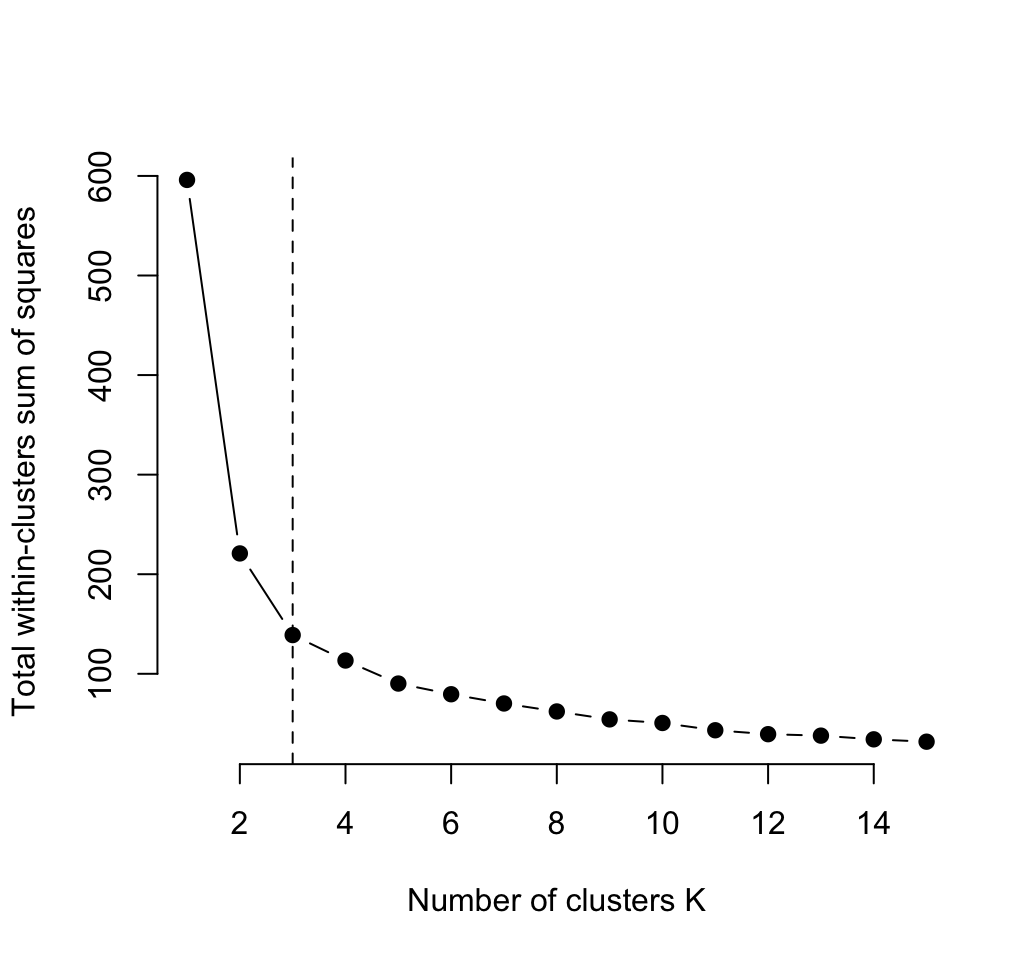
\includegraphics[width=0.8\textwidth]{images/elbow-curve.png}
	\caption{Elbow-Kurve}
	\source{\cite{elbow_method}}
	\label{fig:konzept:parameterauswahl:kprototypes}
\end{figure}

Bei einem Cluster $k=1$ am grössten und wird 0 erreichen wenn $k=n$, wobei $n$ die Anzahl Instanzen darstellt. Der optimale Wert liegt dort wo die Kurve beginnt abzuflachen.

\section{Datenbestand}
\label{sec:recherche:datenbestand}
Nachfolgend wird der Datenbestand und die selektion der Attribute erklärt.

\subsection{Beschreibung der Daten}
\label{sec:recherche:datenbeschaffung}
Die Daten für die Auswertung wurden aus dem \gls{irent} extrahiert werden. Da die Buchungen Kundendaten enthalten, können sie nicht veröffentlicht werden.

Die Daten liegen im Windows Excel Format vor. Es sind total 133'001 Datensätze mit jeweils 153 Felder. Die Zellen A-U sind Informationen im Bezug auf die Buchungen, alle anderen (V-EW) beziehen sich auf das Objekt selber. Die Felbeschreibungen sind im \cref{app:feldbeschreibungen} aufgeführt.

"`boolean"' Datentypen werden behandelt wie "`categorical"' Werte mit nur zwei Ausprägungen, sprich "`0"' und "`1"',

\subsection{Datenvorbereitung}
\label{sec:recherche:datenvorbereitung}
Die Datenvorbereitung wandelt die Daten so um dass sie für das Data Mining möglichst effizient verwendet werden können. Dies umfasst die Bereinigung, Transformation sowie Reduktion von Informationen\footcite{feature_selection_2017-01-04}. Bei ersteren werden Messfehler im Datenbestand behoben, fehlende Felder ergänzt oder Duplikate entfernt. Die Transformation wandelt Werte um damit sie für die Berechnung besser geeignet sind. Zum Beispiel können Wertebereiche in Intervalle aufgeteilt werden. Bei letzteren werden Instanzen der Datengrundlage entfernt, wodurch die Berechnungszeit verkürzt wird, oder Attribute von allen Instanzen entfernt, da deren Entropie zu gering ist. Weiteres hierzu im \cref{sec:proofofconcept:datenvorbereitung} \nameref{sec:proofofconcept:datenveorbereitung}. 

Folgende Modifikationen wurden an den Rohdaten vorgenommen:
\begin{itemize}
\item Das Datenformat wurde für die einfachere programmatische Handhabung von Windows Excel in das \gls{csv}-Format transferiert.
\item Boolsche Werte waren entweder leer (gleichbedeutend mit "`0"') oder "`X"' (gleichbedeutend mit "`1"'). Die Werte wurden geändert auf 0 und 1.
\item Distanzen in den Zeilen AK (Distanz zum Wasser), AL (Distanz zum Skigebiet), AM (Distanz zum öffentlichen Verkehr), DZ (Distanz zum Zentrum), EA (Distanz bis zum Meer) und EB (Distanz bis zum See) wurden diskretisiert. Dabei interessiert es Interhome nur, wenn die Nähe kleiner als 500 ist. Alles über oder gleich 500 wird nicht verwendet. Siehe \cref{fig:recherche:datenvorbereitung:1}.
\item Der Preis wurde diskretisiert. Spannend für die Interpretation sind nur werte welche kleiner als 500 sind oder über 2000. Siehe \cref{fig:recherche:datenvorbereitung:2}.
\end{itemize}

\begin{table}[h] 
	\caption{Diskretisierungswerte für Distanzattribute}
	\centering
	\rowcolors{1}{tablebodycolor}{tablerowcolor}
	\label{fig:recherche:datenvorbereitung:1}
	\begin{tabular}{ | c | c | c | } 
		\hline 
		\rowcolor{tableheadcolor}
		\bfseries Min & \bfseries Max & \bfseries Wert \\ \hline 
		0 & 499 & close \\ \hline 
		500 & $\infty$ &   \\ \hline 
	\end{tabular}
\end{table}

\begin{table}[h] 
	\caption{Diskretisierungswerte des Preises}
	\centering
	\rowcolors{1}{tablebodycolor}{tablerowcolor}
	\label{fig:recherche:datenvorbereitung:2}
	\begin{tabular}{ | c | c | c | } 
		\hline 
		\rowcolor{tableheadcolor}
		\bfseries Min & \bfseries Max & \bfseries Wert \\ \hline 
		0 & 499 & budget \\ \hline 
		500 & 1999 &  \\ \hline 
		2000 & $\infty$ & luxury \\ \hline 
	\end{tabular}
\end{table}

Die Diskretisierung wird durchgeführt, damit nach dem Clustering die Häufigkeit der kategorischen Werte mit dem Apriori Algorithmus erhoben werden kann. Dadurch wird das Clustering nachvollziehbar\todo{cref}\footcite{data_mining_concepts_and_techniques}. 

Es gibt verschiedene Diskretisierungsmethoden. Diese Teilen die Werte in gleiche Intervalle auf oder stellen sicher dass in jeder Kategorie die selbe Anzahl an Instanzen vorhanden sind.
Die verwendeten Werte aus \cref{fig:recherche:datenvorbereitung:1} und \cref{fig:recherche:datenvorbereitung:2} wurde mit Interhome abgesprochen. 

\subsection{Attributeinschränkung}
\label{sec:recherche:attributeinschraenkung}
Der Datenbestand besteht aus 127 Attributen/Spalten. Aus folgenden Gründen sollten die Attribute eingeschränkt werden:
\begin{itemize}
\item Laufzeit der Algorithmen kann durch eine Attributreduktion verbessert werden.
\item Es gibt Attribute welche andere Zusammenfassen. In der \cref{fig:recherche:attributeinschraenkung:1} ist die Zelle "`AW"' eine Aggregation von den darunterliegenden Feldern.
\end{itemize}

\begin{table}[H] 
	\caption{Beispiel eines Attributaggregators}
	\centering
	\rowcolors{1}{tablebodycolor}{tablerowcolor}
		\label{fig:recherche:attributeinschraenkung:1}
	\begin{tabular}{ | c | c | c | l | } 
		\hline 
		\rowcolor{tableheadcolor}
		\bfseries Zelle & \bfseries Name & \bfseries Datentyp & \bfseries Beschreibung \\ \hline 
		AW & CPOOL & boolean & Objekt besitzt einen Pool \\ \hline 
		AX & CPPOOL & boolean & Objekt besitzt einen privaten Pool \\ \hline 
		AY & CHEATED & boolean & Objekt besitzt einen geheizten Pool \\ \hline 
		AZ & CSAFEPOOL & boolean & Objekt besitzt einen sicheren Pool \\ \hline 
		BA & CCHILDPOOL & boolean & Objekt besitzt einen kindersicheren Pool \\ \hline 
		DU & OUTDPOOL & boolean & Objekt besitzt einen aussen Pool \\ \hline 
		DV & INDPOOL & boolean & Objekt besitzt einen innen Pool \\ \hline 
	\end{tabular}
\end{table}

In Absprache mit Interhome wurde entschieden, dass in einem ersten Schritt jene Attribute verwendet werden sollen, welche auch direkt auf der Webseite dargestellt werden. Die zu verendenden Spalten sind in der \cref{fig:recherche:attributeinschraenkung:2} aufgeführt.

\begin{table}[H] 
	\caption{Zu verwendende Attribute}
	\centering
	\rowcolors{1}{tablebodycolor}{tablerowcolor}
		\label{fig:recherche:attributeinschraenkung:2}
	\begin{tabular}{ | c | c | c | l | } 
		\hline 
		\rowcolor{tableheadcolor}
		\bfseries Zelle & \bfseries Name & \bfseries Datentyp & \bfseries Beschreibung \\ \hline 
		E & PRICES & integer & Preis \\ \hline 
		AC & QUAL & integer & Sterne Bewertung des Objektes \\ \hline 
		AD & ROOMS & integer & Anzahl Zimmer \\ \hline 
		AE & BEDROOMS & integer & Anzahl Schlafzimmer \\ \hline 
		AH & PETS & boolean & Haustiere erlaubt? \\ \hline 
		AK & DIWATER & integer & Distanz zum Wasser (m) \\ \hline 
		AL & DISKI & integer & Distanz zum Skigebiet (m) \\ \hline 
		AM & DIPUBT & integer & Distanz zum öffentlichen Verkehr (m) \\ \hline 
		AR & CAIRCOND & boolean & Aircondition im Objekt\\ \hline 
		AW & CPOOL & boolean & Objekt besitzt einen Pool \\ \hline 
		BC & CBBQ & boolean & Objekt besitzt einen Grill \\ \hline 
		BF & CSAUNA & boolean & Objekt besitzt eine Saune \\ \hline 
		BI & CJACUZZI & boolean & Objekt besitzt ein Jacuzzi \\ \hline 
		BM & CWASHMACHI & boolean & Objekt besitzt eine Waschmaschine \\ \hline 
		BU & CPARKING & boolean & Es gibt einen Parkplatz \\ \hline 
		BV & CDISHWASHE & boolean & Objekt besitzt einen Geschirrspühler \\ \hline
		BW & CFIREPLACE & boolean & Objekt besitzt ein Cheminée \\ \hline 
		BX & SCTV & boolean & Objekt besitzt einen Fernseher \\ \hline  
		BY & SCBALCONY & boolean & Objekt besitzt ein Balkon \\ \hline 
		CA & SCNOSMOKE & boolean & Im Objekt darf nicht geraucht werden \\ \hline 
		DZ & DICENTER & integer & Distanz bis zum Zentrum (m) \\ \hline 
		EA & DISEA & integer & Distanz bis zum Meer (m) \\ \hline 
		EB & DILAKE & integer & Distanz bis zum See (m) \\ \hline 
		EG & INTERNET & boolean & Objekt besitzt Internet \\ \hline 
	\end{tabular}
\end{table}

%Einige Attribute sind mehrfach

\subsection{RapidMiner Prozess für die Datenvorbereitung}
\label{sec:konzept:rapidminer}

Die Datenvorbereitung (data preprocessing) wird mit dem Programm RapidMiner durchgeführt.
Zuerst werden die Daten aus dem \gls{csv} File geladen. Anschliessend die Attribute gemäss \cref{fig:recherche:attributeinschraenkung:2} eingeschränkt, die Diskretisierung entsprechend \cref{fig:recherche:datenvorbereitung:1} und \ref{fig:recherche:datenvorbereitung:2} durchgeführt.

\cref{fig:recherche:rapidminer:1} zeigt den Prozess im RapidMiner Studio. In \ref{fig:recherche:rapidminer:1:1} wird der Hauptprozess gezeigt. Zusätzlich sind die Operatoren "`Set Role"' und "`Write CSV"' vorhanden. Ersterer setzt das Feld "`RESNRDIS"' als "`ID"', was intern für RapidMiner benötigt wird. Der letzte Schritt schreibt das Resultat in ein \gls{csv} File damit es nachher weiterverwendet werden kann.

\cref{fig:recherche:rapidminer:1:2} ist ein Unterprozess welcher die Diskretisierung des Preises und der Distanzen vornimmt. Im \cref{sec:recherche:datenvorbereitung} wird beschrieben dass nicht alle Bereich der zu diskretierenden Attribute verwendet werden soll (z.B. Distanzen >499 werden nicht berücksichtigt). Dies kann mit den "`Discretize"' Operatoren in RapidMiner nicht abgebildet werden. Deshalb werden alle Werte diskretiert und die zu ignorierenden nachher entfernt.

\cref{fig:recherche:rapidminer:1:3} zeigt den Unterprozess für die Ersetzung von Attributwerten. Zuerst werden, wie im \cref{sec:recherche:datenbeschaffung} beschrieben, "`X"' Werte von kategorischen Feldern mit "`1"' ersetzt und leere mit "`0"'. Danach werden die nicht zu verwendenden diskretierten Werte der Preise und Distanzen entfernt.

\begin{figure}[htb]
	\begin{subfigure}[t]{1\textwidth}
		\centering
		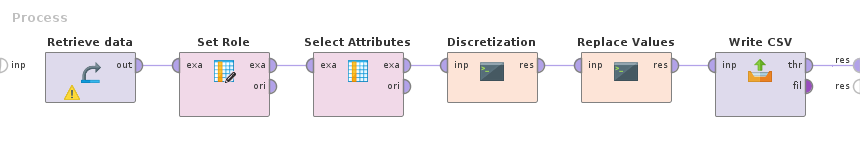
\includegraphics[width=1\textwidth]{images/rapidminer-process}
		\caption{Hauptprocess}
		\label{fig:recherche:rapidminer:1:1}
	\end{subfigure} \\
	\begin{subfigure}[t]{0.5\textwidth}
		\centering
		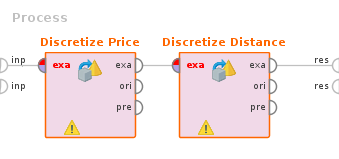
\includegraphics[width=1\textwidth]{images/rapidminer-process-discretization}
		\caption{Subprocess für die Diskretisierung}
		\label{fig:recherche:rapidminer:1:2}
	\end{subfigure}
	\begin{subfigure}[t]{0.8\textwidth}
		\centering
		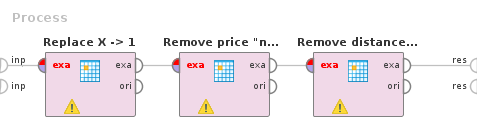
\includegraphics[width=1\textwidth]{images/rapidminer-process-replace-values}
		\caption{Subprocess für die Ersetzung von Attributwerten}
		\label{fig:recherche:rapidminer:1:3}
	\end{subfigure}
	\caption{RapidMiner Prozess für die Vorbereitung der Daten}
	\label{fig:recherche:rapidminer:1}
\end{figure}

\section{Ablauf}
Der Ablauf des Data Mining im zu entwickelnden Programm ist zweistufig. Als erstes gibt der User eine Abfrage ein, für welche anschliessend eine eine Liste von häufig auftretenden Attributen gesucht werden soll (siehe \cref{sec:einletung:ziel} \nameref{sec:einletung:ziel}).


\subsection{Einschränkung des Datenbestandes}
Im ersten Schritt wird der Datenbestand durch die Auswahl von Attributen durch den Benutzer eingeschränkt. Er kann 0-n Werte aus den in der \cref{fig:recherche:attributeinschraenkung:2} gelisteten Attributen selektieren. Anschliessend werden alle Instanzen aus der Datenmenge entfernt welche den Kriterien nicht genügen. Dies bildet die Grundlage für die Analyse im Schritt 2.

\subsection{Auffinden von Attributen}
Für den zweiten Schritt wird entweder ein \nameref{sec:konzept:disziplinauswahl:association} (siehe \cref{sec:konzept:disziplinauswahl:association}) oder eine \nameref{sec:konzept:disziplinauswahl:clusteranalysis} (siehe \cref{sec:konzept:disziplinauswahl:clusteranalysis}) durchgeführt. 

Möchte der Benutzer wissen, welche Attribute in der vor-selektierten Datenmenge oft vorkommen, so kann der Apriori-Algorithmus gewählt werden. Liefert dieser keine zufriedenstellenden Antworten oder ist von vornherein zu erwarten, dass es verschiedene Gruppen von Buchungen gibt, so kann zuerst die Cluster Analysis durchgeführt werden. Die Instanzen werden damit in Clusters/Klassen aufgeteilt, der Benutzer würde jedoch nicht sehen weshalb. Deshalb wird auf jeder Klasse der Apriori-Algorithmus durchgeführt. Da die Instnzen in einer Klasse untereinander möglichst Homogen sein sollen und möglichst unterschiedlich zu anderen Clusters, ist anzunehmen, dass die häufigsten Attribute, welche durch den Apriori-Algorithmus gefunden werden, aussagekräftig die Klassen beschreiben.

\section{Mockups des Programmes}
\label{sec:konzept:mockups}
Die graphischen Oberfläche des Programmes wird nachfolgend anhand von Mockups aufgezeigt. Die Auflistung der Stammdaten sowie der Resultate ist einfachheitshalber verkürzt dargestellt. Auf jeder Seite zuoberst ist das Interhome Logo sowie die Navigation platziert.

In \cref{fig:konzept:mockups:stammdaten} ist die Startseite abgebildet in welcher der Benutzer die Stammdaten (FA4) einsehen kann. Im oberen Bereich sind die Filter, mit welchen der Datenbestand eingeschränkt werden kann. 
\begin{figure}[H]
	\RawFloats
	\centering
	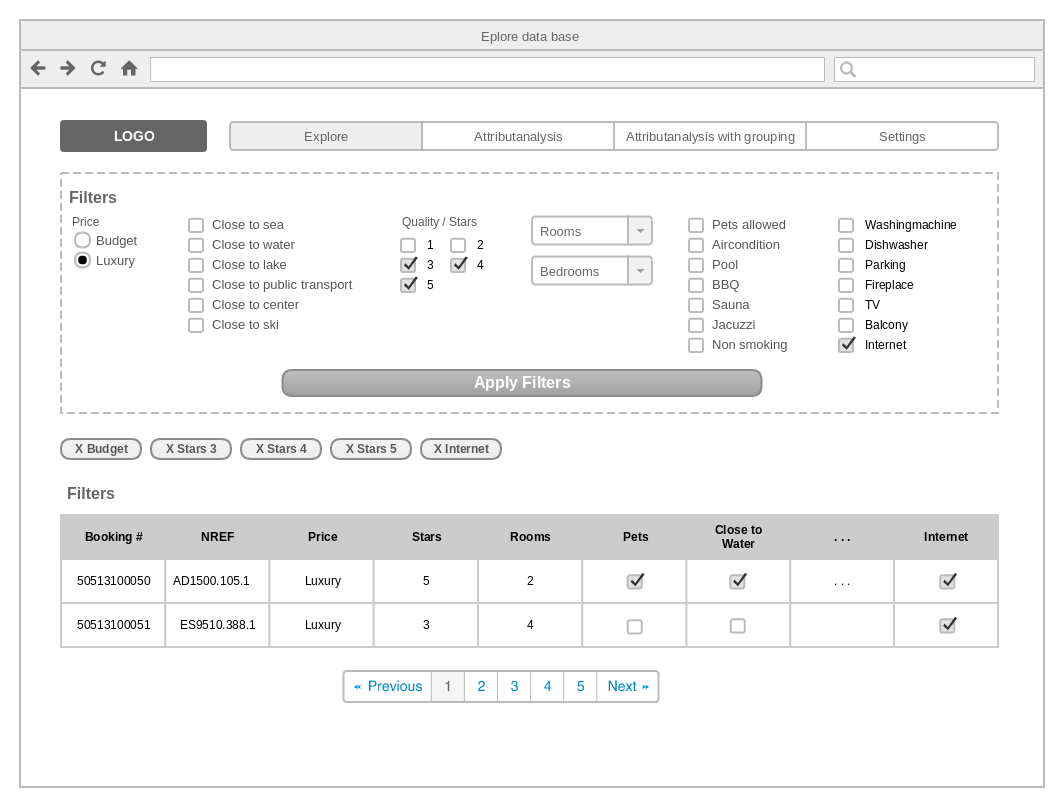
\includegraphics[width=1\textwidth]{images/wireframe-explore}
	\caption{Mockup für das einsehen der Stammdaten (FA4)}
	\label{fig:konzept:mockups:stammdaten}
\end{figure}

Auf der zweiten Seite, welche in \cref{fig:konzept:mockups:apriori} dargestellt ist, kann der Benutzer eine apriori Analyse durchführen (siehe \cref{sec:konzept:algorithmenauswahl:apriori} \nameref{sec:konzept:algorithmenauswahl:apriori}). Wie vorher sind zuoberst die selben Filter plaziert. Darunter sind die Attribute aufgelistet, welche vom Algorithmus gefunden wurde sowie deren Häufigkeit. Zuunterst ist zur Kontrolle noch der analysierte Datenbestand aufgeführt.
\begin{figure}[H]
	\RawFloats
	\centering
	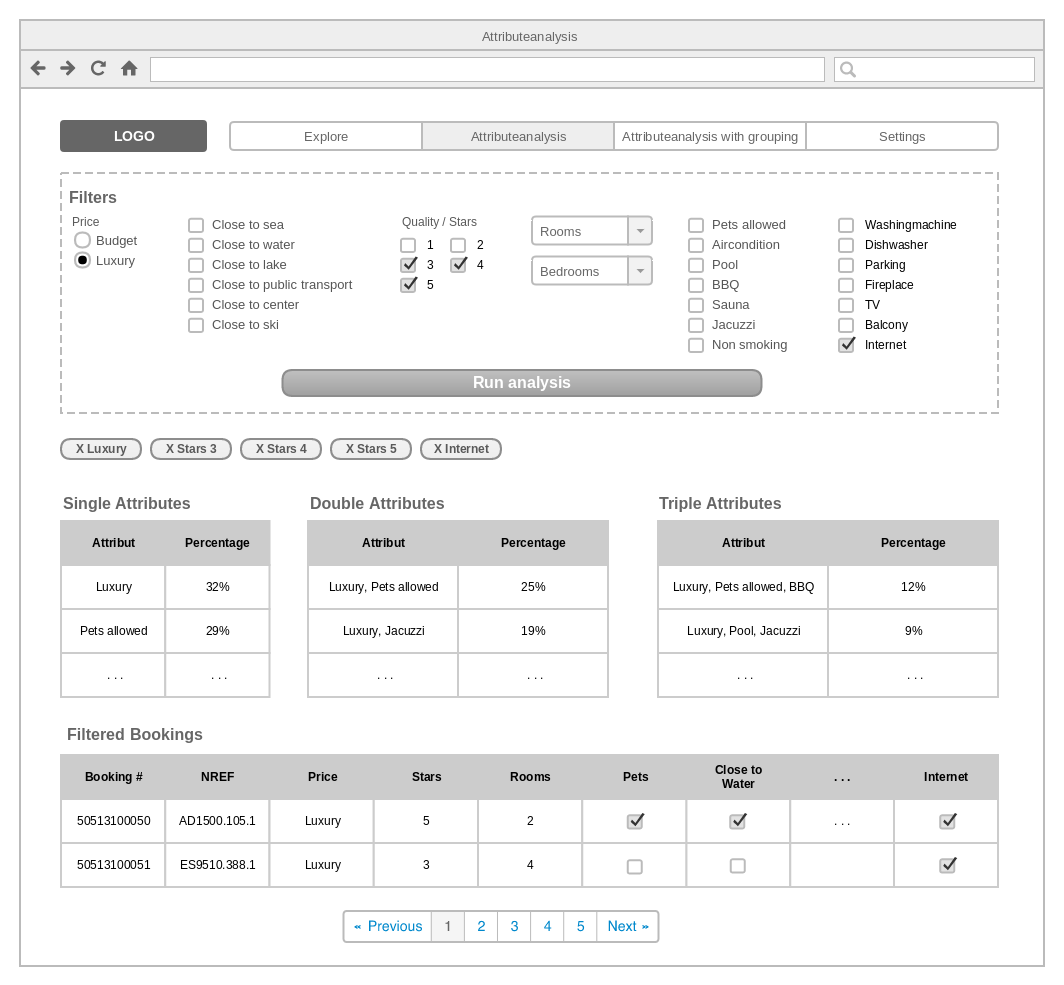
\includegraphics[width=1\textwidth]{images/wireframe-apriori}
	\caption{Mockup für die Analyse mit dem apriori Algorithmus}
	\label{fig:konzept:mockups:apriori}
\end{figure}

Der dritte Reiter führt zur Analyse mit den Clustering Algorithmen k-prototypes und DBSCAN (\cref{sec:konzept:algorithmenauswahl:clustering} \nameref{sec:konzept:algorithmenauswahl:clustering}). Die Filter sind entsprechend den vorherigen Seite zuoberst platziert. Es gibt jedoch zwei Buttons um die Analyse mit den entsprechenden Algorithmen zu starten. Zuunterst sind die gefunden Clusters abgebildet, mit den häufigen Attributen sowie den Buchungen, welche zu den entsprechenden Clustern gehören. Zur Verbesserung der Übericht können die Bereiche auf- und zugeklappt werden.

\begin{figure}[H]
	\RawFloats
	\centering
	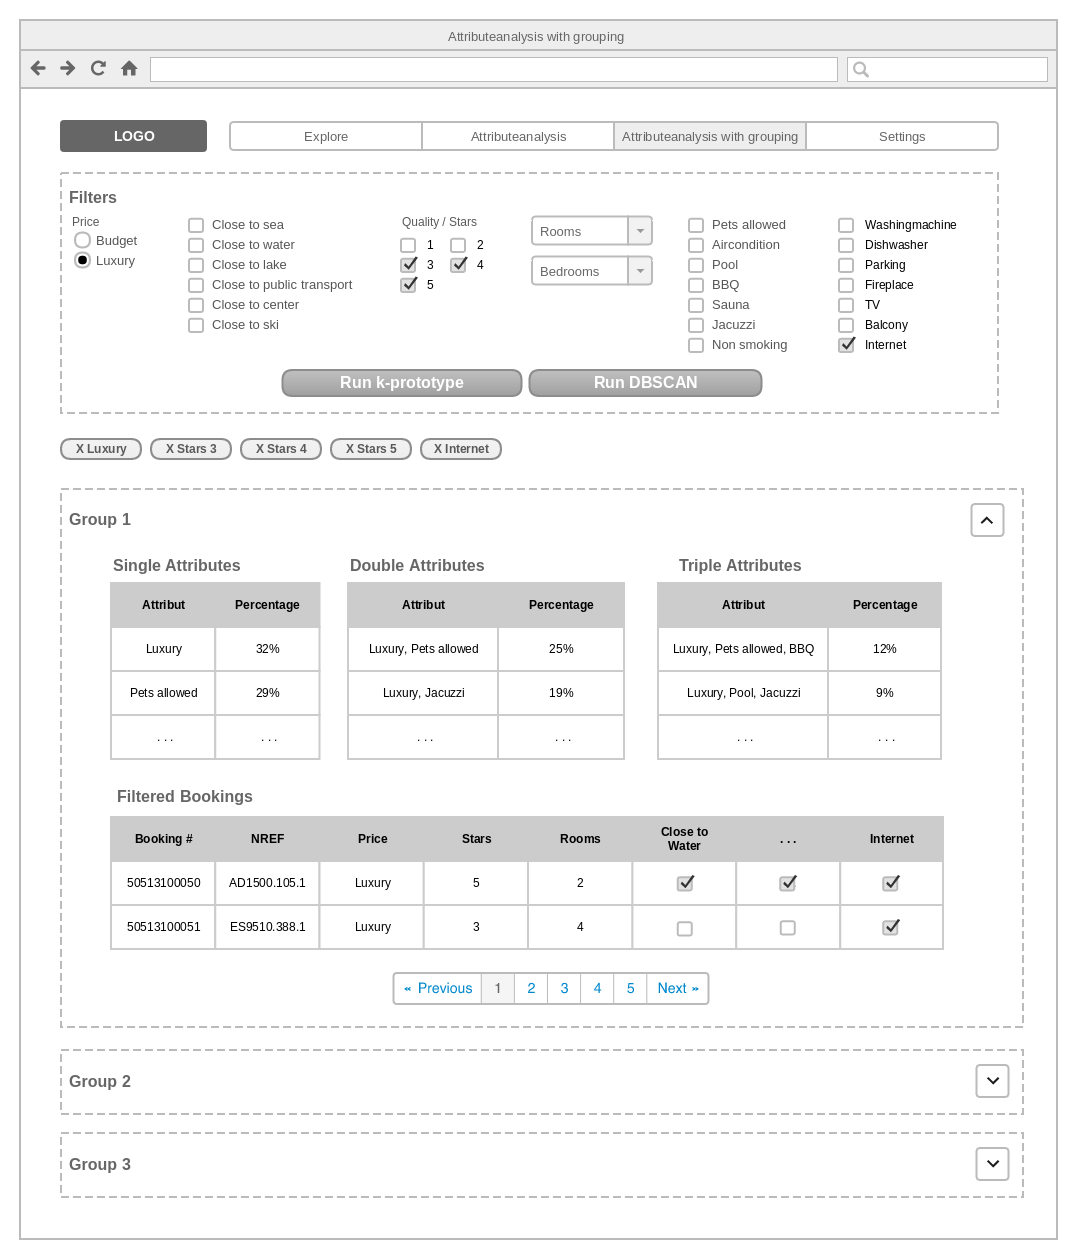
\includegraphics[width=1\textwidth]{images/wireframe-clustering}
	\caption{Mockup für die Analyse mit dem apriori Algorithmus}
	\label{fig:konzept:mockups:apriori}
\end{figure}

\section{Testcases}
\label{sec:recherche:testcases}
